% Baccalauréat malgache, série C, 2014 : corrigé.
\TCDBacAttribution{C}{2014}
\providecommand{\cm}{~\mathrm{cm}}
\providecommand{\dx}{~\mathrm{d}x}
\providecommand{\dt}{\mathrm{d}t}
\providecommand{\mes}[2]{\mathrm{mes}\left( \widehat{ \overrightarrow{#1} ; \overrightarrow{#2} } \right)}
\providecommand{\Angl}[2]{\left( \widehat{ \overrightarrow{#1} , \overrightarrow{#2} } \right)}
%
%%%%%%%%%%%%%%%%%%%%%%%%%%%%%%%%%%%%%%%%%%%%%%%%%%%%%%%%%%%%%%%%%%%%%%%%%%%%%%%%%%%%%%%%%%%%%%%%%%%%%%%%%%%%%%%%%%%%%%%%%%%%%%%%
\noindent \underline{\textsc{\textbf{Exercice}}} (4 points)
\begin{description}
	\item[Partie A]
	\begin{enumerate}
		\item \vln{Calcul de $P_A$ et $P_B$ :}
			Les trois zones forment une partition des issues : $P_A + P_B + P_C = 1$.
			En progression arithmétique, $P_A + P_C = 2P_B$, donc $3P_B = 1$ : $P_B = \frac{1}{3}$, puis $P_A = 2P_B - P_C = \frac{2}{3} - \frac{1}{6}$.
			\par\noindent\ansbox{$P_A = \frac{1}{2}$ et $P_B = \frac{1}{3}$.}
		\item \vln{Au moins une fois la zone C en quatre tirs :}
			L'événement contraire est « ne jamais atteindre C » ; les tirs sont indépendants :
			$1 - \left(\frac{5}{6}\right)^4 = 1 - \frac{625}{1296}$, soit \par\noindent\ansbox{$\frac{671}{1296} \approx 0{,}52$.}
		\item \vln{Événement $E$ :}
			Le jeu s'arrête au $3^{\text{e}}$ tir si les deux premiers tirs manquent C et le troisième l'atteint :
			$P(E) = \left(\frac{5}{6}\right)^2 \times \frac{1}{6}$, soit \par\noindent\ansbox{$P(E) = \frac{25}{216}$.}
		\item \vln{Probabilité $P_n$ :}
			De même, $n - 1$ échecs puis un succès :
			\par\noindent\ansbox{$P_n = \frac{1}{6}\left(\frac{5}{6}\right)^{n-1}$ et $\lim_{n\to+\infty} P_n = 0$ (car $0 < \frac{5}{6} < 1$).}
	\end{enumerate}
	\item[Partie B]
	\begin{enumerate}
		\item \vln{Divisibilités :}
			$(x + 6y)^2 - x^2 = 12xy + 36y^2 = 12\left(xy + 3y^2\right)$ : divisible par $12$.
			$(x + 6y)^4 - x^4 = \left[(x+6y)^2 - x^2\right]\left[(x+6y)^2 + x^2\right]$. Le second facteur est pair :
			$(x + 6y)^2 + x^2 = 2x^2 + 12xy + 36y^2 = 2\left(x^2 + 6xy + 18y^2\right)$.
			Le produit est donc divisible par $12 \times 2 = 24$.
			\par\noindent\ansbox{$12$ divise $(x+6y)^2 - x^2$ et $24$ divise $(x+6y)^4 - x^4$.}
		\item \vln{Résolution de $3x \equiv 2 \ [7]$ :}
			$3 \times 5 = 15 \equiv 1 \ [7]$ ; en multipliant par $5$ : $x \equiv 10 \equiv 3 \ [7]$. Réciproquement $3 \times 3 = 9 \equiv 2$.
			\par\noindent\ansbox{$x = 3 + 7k$, $k \in \mathbb{Z}$.}
		\item \vln{Base $b$ :}
			Le chiffre $4$ impose $b \geq 5$. $(b + 2)(2b + 2) = 3b^2 + b + 4 \iff 2b^2 + 6b + 4 = 3b^2 + b + 4 \iff b^2 - 5b = 0$.
			\par\noindent\ansbox{$b = 5$} (vérification : $7 \times 12 = 84 = 3 \times 25 + 1 \times 5 + 4$).
	\end{enumerate}
\end{description}
%%%%%%%%%%%%%%%%%%%%%%%%%%%%%%%%%%%%%%%%%%%%%%%%%%%%%%%%%%%%%%%%%%%%%%%%%%%%%%%%%%%%%%%%%%%%%%%%%%%%%%%%%%%%%%%%%%%%%%%%%%%%%%%%
\noindent \underline{\textsc{\textbf{PROBLEME I}}} (7 points) \newline
Comme sur la figure de l'énoncé, $I$ est le milieu de $[OA]$ (c'est ce qu'impose $\vec{u} = \overrightarrow{OI}$ dans la partie II et les codages de la figure).
Les triangles $AOE$, $BAC$, $OBD$ étant directs et rectangles isocèles en $E$, $C$, $D$ : $\Angl{EA}{EO} = \Angl{CB}{CA} = \Angl{DO}{DB} = \frac{\pi}{2}$.
\begin{center}
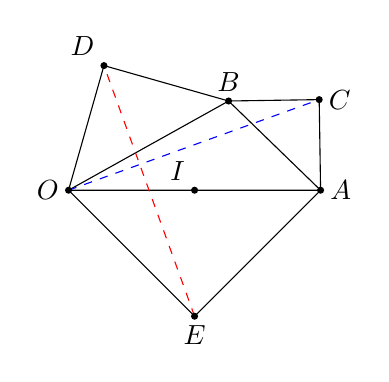
\begin{tikzpicture}[scale=1.6]
	\coordinate (O) at (0,0); \coordinate (A) at (2,0); \coordinate (I) at (1,0); \coordinate (E) at (1,-1);
	\coordinate (B) at (1.27,0.708); \coordinate (C) at (1.989,0.719); \coordinate (D) at (0.281,0.989);
	\draw (O) -- (A) -- (B) -- cycle;
	\draw (O) -- (E) -- (A); \draw (B) -- (C) -- (A); \draw (O) -- (D) -- (B);
	\draw[blue,dashed] (O) -- (C); \draw[red,dashed] (E) -- (D);
	\foreach \P/\pos in {O/left,A/right,I/above left,E/below,B/above,C/right,D/above left}
		\fill (\P) circle (0.8pt) node[\pos] {$\P$};
\end{tikzpicture}
\end{center}
\begin{description}
	\item[PARTIE I :] Méthode 1.
	\begin{enumerate}
		\item
		\begin{enumerate}
			\item \vln{Rapports et angles :}
				Dans le triangle $BAC$ rectangle isocèle en $C$, $AB = \sqrt{2}\,AC$ et l'angle en $A$ vaut $\frac{\pi}{4}$ ; le triangle étant direct, $\Angl{AC}{AB} = \frac{\pi}{4}$.
				\par\noindent\ansbox{$S_1$ : centre $A$, rapport $\sqrt{2}$, angle $\frac{\pi}{4}$.}
				Dans $OBD$ rectangle isocèle en $D$, $OD = \frac{OB}{\sqrt{2}}$ et $\Angl{OB}{OD} = \frac{\pi}{4}$.
				\par\noindent\ansbox{$S_2$ : centre $O$, rapport $\frac{\sqrt{2}}{2}$, angle $\frac{\pi}{4}$.}
			\item \vln{Nature de $f$ :}
				$f = S_2 \circ S_1$ est une similitude directe de rapport $\sqrt{2} \times \frac{\sqrt{2}}{2} = 1$ et d'angle $\frac{\pi}{4} + \frac{\pi}{4} = \frac{\pi}{2}$ :
				un déplacement d'angle non nul.
				\par\noindent\ansbox{$f$ est une rotation d'angle $\frac{\pi}{2}$.}
		\end{enumerate}
		\item \vln{Images de $I$ et de $E$ :}
			Dans le triangle $AOE$ rectangle isocèle en $E$, la médiane $[EI]$ est aussi hauteur et $IE = IA = IO$ ; ainsi $AEI$ est rectangle isocèle en $I$,
			avec $AE = \sqrt{2}\,AI$ et $\Angl{AI}{AE} = \frac{\pi}{4}$ (sens direct, comme $AOE$). Donc $S_1(I) = E$.
			De même $OE = \sqrt{2}\,OI$ et $\Angl{OE}{OI} = \frac{\pi}{4}$, donc $OI = \frac{\sqrt{2}}{2}OE$ et $S_2(E) = I$.
			\par\noindent\ansbox{$S_1(I) = E$, $S_2(E) = I$, donc $f(I) = S_2(E) = I$ : $I$ est invariant par $f$.}
			$f$ est donc la rotation de centre $I$ et d'angle $\frac{\pi}{2}$, c'est-à-dire $f = R$.
		\item
		\begin{enumerate}
			\item \vln{$R(O)$ et $R(C)$ :}
				$IO = IE$ et $\Angl{IO}{IE} = \frac{\pi}{2}$ (triangle $OIE$ rectangle isocèle en $I$, de sens direct), donc $R(O) = E$.
				$R(C) = f(C) = S_2(S_1(C)) = S_2(B) = D$.
				\par\noindent\ansbox{$R(O) = E$ et $R(C) = D$.}
			\item \vln{Conclusion :}
				La rotation $R$ transforme le segment $[OC]$ en $[ED]$ : $ED = OC$ et $\Angl{OC}{ED} = \frac{\pi}{2}$.
				\par\noindent\ansbox{$(OC) \perp (ED)$ et $OC = ED$.}
		\end{enumerate}
	\end{enumerate}
	\item[PARTIE II :] Méthode 2. On a $z_O = 0$, $z_I = 1$, $z_A = 2$, $z_B = b$.
	\begin{enumerate}
		\item \vln{Affixes de $C$ et $D$ :}
			$\Angl{CB}{CA} = \frac{\pi}{2}$ et $CA = CB$ : $z_A - z_C = i(b - z_C)$, d'où $z_C(i - 1) = ib - 2$ et
			$z_C = \frac{ib - 2}{i - 1} = \frac{(ib - 2)(-1 - i)}{2} = \frac{(1 - i)b + 2 + 2i}{2}$.
			$\Angl{DO}{DB} = \frac{\pi}{2}$ et $DO = DB$ : $b - z_D = i(0 - z_D)$, d'où $z_D(1 - i) = b$ et $z_D = \frac{b}{1 - i} = \frac{(1+i)b}{2}$.
			\par\noindent\ansbox{$Z_C = \frac{(1-i)\,b}{2} + 1 + i$ et $Z_D = \frac{(1+i)\,b}{2}$.}
		\item \vln{Affixe de $E$ :}
			$z_A - Z_E = i(0 - Z_E)$, d'où $Z_E(1 - i) = 2$ et \par\noindent\ansbox{$Z_E = \frac{2}{1-i} = 1 - i$.}
		\item
		\begin{enumerate}
			\item \vln{Quotient :}
				$i(Z_C - Z_O) = \frac{(i + 1)b}{2} + i - 1 = Z_D - (1 - i) = Z_D - Z_E$ ; et $Z_C \neq 0$ dès que $C \neq O$ (cas de la figure ; le cas $C = O$, qui correspond à $b = -2i$, donne aussi $D = E$).
				\par\noindent\ansbox{$\frac{Z_D - Z_E}{Z_C - Z_O} = i$.}
			\item \vln{Conclusion :}
				$|i| = 1$ donne $ED = OC$ et $\arg i = \frac{\pi}{2}$ donne $\Angl{OC}{ED} = \frac{\pi}{2}$.
				\par\noindent\ansbox{$(OC) \perp (ED)$ et $OC = ED$.}
		\end{enumerate}
	\end{enumerate}
\end{description}
%%%%%%%%%%%%%%%%%%%%%%%%%%%%%%%%%%%%%%%%%%%%%%%%%%%%%%%%%%%%%%%%%%%%%%%%%%%%%%%%%%%%%%%%%%%%%%%%%%%%%%%%%%%%%%%%%%%%%%%%%%%%%%%%
\noindent \underline{\textsc{\textbf{PROBLEME II}}} (9 points)
\begin{description}
	\item[PARTIE I :]
	\begin{enumerate}
		\item \vln{Continuité en $1$ :}
			$f(1) = 0 + \ln\frac{2}{2} = 0$ ; $\lim_{x\to 1^-} (1 - x)\expo{x} = 0$ ; à droite, $f$ est continue sur $[1;+\infty[$.
			\par\noindent\ansbox{$f$ est continue en $1$.}
		\item
		\begin{enumerate}
			\item \vln{Dérivabilité à droite :}
				Pour $x > 1$ : $\ln\frac{2x}{x+1} = \ln 2 + \ln x - \ln(x+1)$, donc
				$\frac{f(x) - f(1)}{x - 1} = \frac{x - 1 + \ln x - \left(\ln(x+1) - \ln 2\right)}{x - 1} = 1 + \frac{\ln x}{x - 1} - \frac{\ln(x+1) - \ln 2}{x - 1}$.
				Or $\frac{\ln x - \ln 1}{x - 1} \to (\ln)'(1) = 1$ et $\frac{\ln(x+1) - \ln 2}{x - 1}$ tend vers la dérivée de $x \mapsto \ln(x+1)$ en $1$, soit $\frac{1}{2}$.
				\par\noindent\ansbox{$f$ est dérivable à droite en $1$ et $f'_d(1) = 1 + 1 - \frac{1}{2} = \frac{3}{2}$.}
			\item \vln{Dérivabilité à gauche :}
				Pour $x < 1$ : $\frac{f(x) - f(1)}{x - 1} = \frac{(1 - x)\expo{x}}{x - 1} = -\expo{x} \to -e$.
				\par\noindent\ansbox{$f$ est dérivable à gauche en $1$ avec $f'_g(1) = -e$ ; $f$ n'est pas dérivable en $1$ (point anguleux).}
		\end{enumerate}
		\item \vln{Limites :}
			En $-\infty$ : $(1 - x)\expo{x} = \expo{x} - x\expo{x} \to 0 - 0$. En $+\infty$ : $\frac{2x}{x+1} \to 2$, donc $\ln\frac{2x}{x+1} \to \ln 2$ et $x - 1 \to +\infty$.
			\par\noindent\ansbox{$\lim_{x\to-\infty} f(x) = 0$ et $\lim_{x\to+\infty} f(x) = +\infty$.}
		\item
		\begin{enumerate}
			\item \vln{Sens de variation :}
				Sur $]-\infty;1[$ : $f'(x) = -\expo{x} + (1 - x)\expo{x} = -x\expo{x}$ : positive sur $]-\infty;0[$, négative sur $]0;1[$.
				Sur $]1;+\infty[$ : $f'(x) = 1 + \frac{1}{x} - \frac{1}{x+1} = 1 + \frac{1}{x(x+1)} > 0$.
				\par\noindent\ansbox{$f$ est croissante sur $]-\infty;0]$, décroissante sur $[0;1]$, croissante sur $[1;+\infty[$.}
			\item \vln{Tableau de variation :}
				\[
				\begin{array}{c|ccccccc}
					x & -\infty & & 0 & & 1 & & +\infty \\ \hline
					f'(x) & & + & 0 & - & -e \,\|\, \frac{3}{2} & + & \\ \hline
					 & & & 1 & & & & +\infty \\
					f & & \nearrow & & \searrow & & \nearrow & \\
					 & 0 & & & & 0 & &
				\end{array}
				\]
		\end{enumerate}
		\item \vln{Limite de $\varphi$ :}
			Pour $x \geq 1$ : $\varphi(x) = \ln\frac{2x}{x+1} - \ln 2 = \ln\frac{x}{x+1} \to \ln 1 = 0$.
			\par\noindent\ansbox{$\lim_{x\to+\infty}\varphi(x) = 0$ : la droite $\Delta : y = x - 1 + \ln 2$ est asymptote à $(C)$ en $+\infty$.}
			De plus $\frac{x}{x+1} < 1$, donc $\varphi(x) < 0$ : $(C)$ est en dessous de $\Delta$. En $-\infty$, l'axe des abscisses est asymptote.
		\item \vln{Tracé (unité $1\cm$) :}
			Demi-tangentes en $(1;0)$ : à gauche de pente $-e$, à droite de pente $\frac{3}{2}$. Valeurs : $f(-2) \approx 0{,}41$ ; $f(-1) \approx 0{,}74$ ; $f(0) = 1$ ; $f(2) \approx 1{,}29$ ; $f(4) \approx 3{,}47$.
			\begin{center}
			\begin{tikzpicture}[x=1cm,y=1cm,>=stealth]
				\draw[->] (-5.5,0) -- (6,0) node[below] {$x$};
				\draw[->] (0,-1.2) -- (0,5.5) node[left] {$y$};
				\foreach \t in {-5,-4,-3,-2,-1,1,2,3,4,5} \draw (\t,0.05) -- (\t,-0.05) node[below] {\small $\t$};
				\foreach \t in {1,2,3,4,5} \draw (0.05,\t) -- (-0.05,\t) node[left] {\small $\t$};
				\draw[red] (0.3,-1) -- (5.8,4.5) node[right] {$\Delta$};
				\draw[blue,thick] plot[domain=-5.5:1,samples=100] (\x,{(1-\x)*exp(\x)});
				\draw[blue,thick] plot[domain=1:5.8,samples=80] (\x,{\x-1+ln(2*\x/(\x+1))});
				\draw[gray] (0.7,0.815) -- (1,0) -- (1.5,0.75);
				\node[blue] at (-2.5,1) {$(C)$};
			\end{tikzpicture}
			\end{center}
	\end{enumerate}
	\item[PARTIE II :]
	\begin{enumerate}
		\item \vln{Équation différentielle :}
			$\varphi'(x) = -\expo{-x}g(x) + \expo{-x}g'(x) = \expo{-x}\left(g'(x) - g(x)\right) = \expo{-x}(-2x + 1)\expo{x}$, donc
			\par\noindent\ansbox{$\varphi'(x) = -2x + 1$.}
			Ainsi $\varphi(x) = -x^2 + x + k$, $k \in \mathbb{R}$, et $g(x) = \expo{x}\varphi(x) = (-x^2 + x + k)\expo{x}$
			(réciproquement ces fonctions sont solutions, le calcul précédent étant réversible). $g(0) = k = 1$ :
			\par\noindent\ansbox{$g(x) = (-x^2 + x + 1)\expo{x}$.}
		\item \vln{Équation trigonométrique :}
			$\sqrt{3}\cos x + \sin x = 2\left(\frac{\sqrt{3}}{2}\cos x + \frac{1}{2}\sin x\right) = 2\cos\left(x - \frac{\pi}{6}\right)$.
			L'équation devient $\cos\left(x - \frac{\pi}{6}\right) = \frac{\sqrt{2}}{2} = \cos\frac{\pi}{4}$, soit $x - \frac{\pi}{6} = \pm\frac{\pi}{4} + 2k\pi$ :
			$x = \frac{5\pi}{12} + 2k\pi$ ou $x = -\frac{\pi}{12} + 2k\pi$.
			\par\noindent\ansbox{Dans $[0;2\pi]$ : $S = \left\{\frac{5\pi}{12} \, ; \frac{23\pi}{12}\right\}$.}
		\item
		\begin{enumerate}
			\item \vln{Calcul de $I_1$ :}
				Par parties ($u = 1 - x$, $v' = \expo{x}$) : $I_1 = \left[(1-x)\expo{x}\right]_0^1 + \int_0^1 \expo{x}\dx = -1 + (e - 1)$.
				\par\noindent\ansbox{$I_1 = e - 2 \approx 0{,}72$.}
				Sur $[0;1]$, $f(x) = (1 - x)\expo{x} \geq 0$ : $I_1$ est l'aire, en $\mathrm{cm}^2$ (unité $1\cm$), du domaine limité par $(C)$, l'axe des abscisses et les droites $x = 0$ et $x = 1$.
			\item \vln{Relation de récurrence :}
				Par parties avec $u = (1 - x)^{n+1}$, $v' = \expo{x}$ :
				$\int_0^1 (1-x)^{n+1}\expo{x}\dx = \left[(1-x)^{n+1}\expo{x}\right]_0^1 + (n+1)\int_0^1 (1-x)^n\expo{x}\dx = -1 + (n+1)\,n!\,I_n$.
				En divisant par $(n+1)!$ : \par\noindent\ansbox{$I_{n+1} = I_n - \frac{1}{(n+1)!}$.}
				Par récurrence : $I_1 = e - 2 = e - 1 - \frac{1}{1!}$ ; si $I_n = e - 1 - \sum_{k=1}^{n}\frac{1}{k!}$, alors $I_{n+1} = e - 1 - \sum_{k=1}^{n+1}\frac{1}{k!}$.
				\par\noindent\ansbox{$I_n = e - 1 - \sum_{k=1}^{n}\frac{1}{k!}$ pour tout $n \geq 1$.}
			\item \vln{Encadrement et limite :}
				Sur $[0;1]$, $1 \leq \expo{x} \leq e$ et $(1 - x)^n \geq 0$ ; or $\int_0^1 (1-x)^n\dx = \frac{1}{n+1}$. Donc
				$\frac{1}{n!}\cdot\frac{1}{n+1} \leq I_n \leq \frac{e}{n!}\cdot\frac{1}{n+1}$ :
				\par\noindent\ansbox{$\frac{1}{(n+1)!} \leq I_n \leq \frac{e}{(n+1)!}$.}
				Comme $\frac{e}{(n+1)!} \to 0$, $I_n \to 0$, d'où
				\par\noindent\ansbox{$\lim_{n\to+\infty}\sum_{k=1}^{n}\frac{1}{k!} = e - 1$.}
		\end{enumerate}
	\end{enumerate}
\end{description}
